\begin{wrapfigure}[0]{r}[0cm]{4cm}
 \vspace{-6cm}
  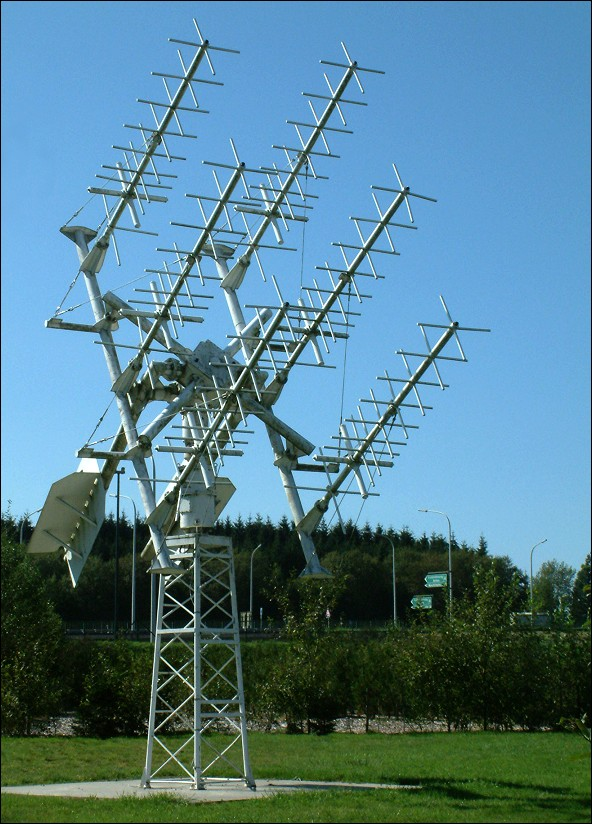
\includegraphics[scale=0.2]{Antennen/Bilder/Kreuzdipolarp.jpg}
 \vspace{-6cm}
\end{wrapfigure}

\section*{Theorie- und Prüfungsfragen}

%--------------------------------------------

\begin{enumerate} 
\itemsep1pt\parskip0pt\parsep0pt
\item[1] Ordne der Abbildungen mit Schleifenantennen \ref{schleifen} folgende Bauformen zu: Dreiecksschleife (Delta Loop), Faltdipol, Quadratische Schleife (Quad Loop)
\loesung{
    Bild A zeigt einen Faltdipol.
    Bild B zeigt eine  Quadratische Schleife (Quad Loop).
    Bild C zeigt eine Dreiecksschleife (Delta Loop).
}
\end{enumerate}

\begin{figure}[H]
	\centering
	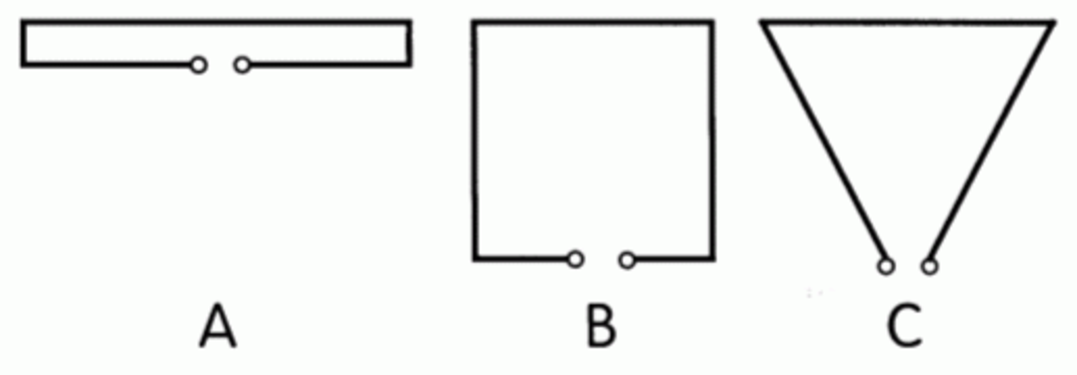
\includegraphics[scale=0.4]{Antennen/Bilder/Schleifen.pdf}
	\caption{Bauformen von Schleifenantennen}
	\label{schleifen}
\end{figure}

%--------------------------------------------

\begin{enumerate} 
\itemsep1pt\parskip0pt\parsep0pt
\item[2] Ordne der Abbildungen mit UKW-Vertikalantennen \ref{ukw} folgende Bauformen zu: Groundplane-Antenne, Sperrtopf-Antenne, Viertelwellenstab, $\lambda/2$-Antenne, $5/8- \lambda$-Antenne
\loesung{
    Bild A zeigt einen Viertelwellenstab.
    Bild B zeigt eine  $\lambda/2$-Antenne.
    Bild C zeigt eine $5/8- \lambda$-Antenne.
    Bild D zeigt eine Sperrtopf-Antenne.
    Bild E zeigt eine Groundplane-Antenne.
}
\end{enumerate}

\begin{figure}[H]
	\centering
	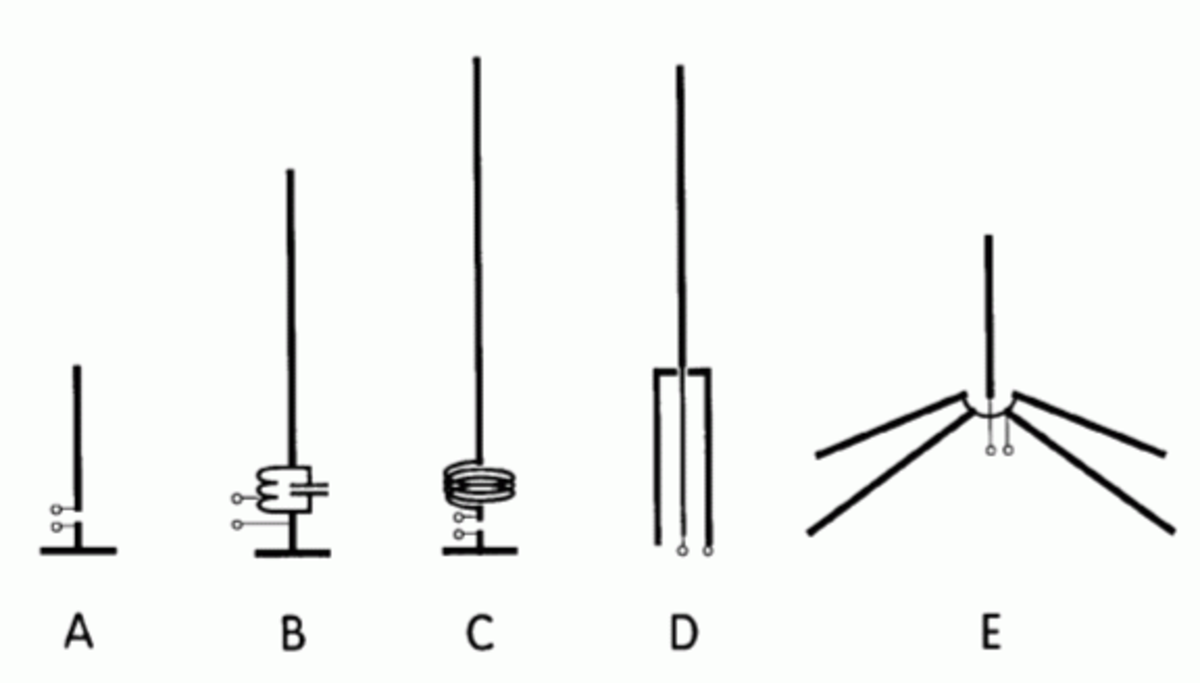
\includegraphics[scale=0.4]{Antennen/Bilder/ukw.pdf}
	\caption{Bauformen von UKW-Vertikalantennen}
	\label{ukw}
\end{figure}

%--------------------------------------------


\begin{enumerate} 
\itemsep1pt\parskip0pt\parsep0pt
\item[3] Ordne der Abbildungen \ref{yagi} folgende Bauformen zu: horizontal polarisierte Yagi-Antenne, zirkular polarisierte X-Yagi-Antenne, Kreuz-Yagi-Antenne, vertikal polarisierte Yagi-Antenne.
\loesung{
    Bild A zeigt eine horizontal polarisierte Yagi-Antenne.
    Bild B zeigt eine vertikal polarisierte Yagi-Antenne.
    Bild C zeigt eine Kreuz-Yagi-Antenne.
    Bild D zeigt eine zirkular polarisierte X-Yagi-Antenne.
}
\end{enumerate}

\begin{figure}[H]
	\centering
	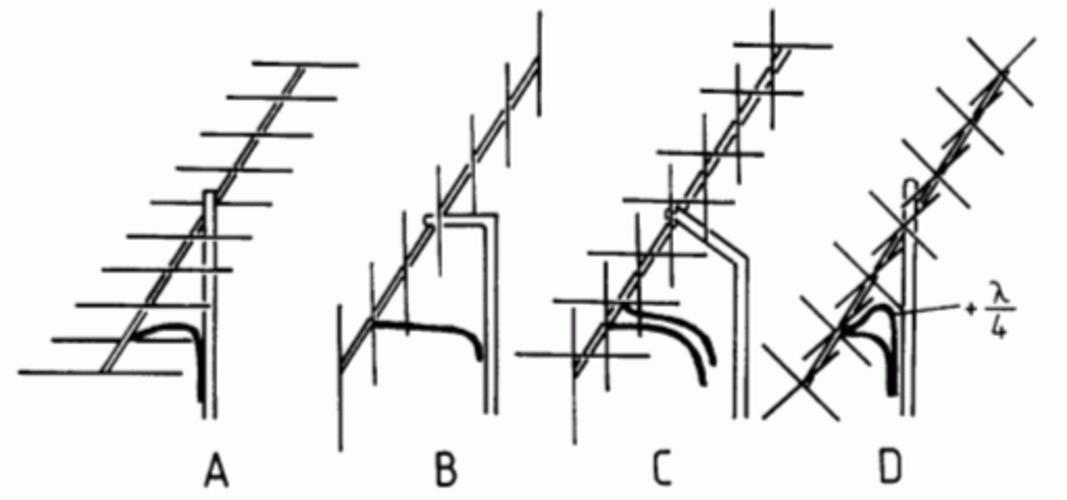
\includegraphics[scale=0.4]{Antennen/Bilder/TH209.pdf}
	\caption{Bauformen von Yagi-Antennen}
	\label{yagi}
\end{figure}
%------------------------------------------------------
\begin{enumerate} 
\itemsep1pt\parskip0pt\parsep0pt
\item[4] Ordne den Abbildungen \ref{strahlungsdiagramm} folgende Strahlungsdiagramme zu: Groundplane, Yagi-Antenne, Dipol, gibt es nicht.
\loesung{
    Bild A Dipol
    Bild B Yagi-Antenne
    Bild C Groundplane
    Bild D gibt es nicht
}
\end{enumerate}

\begin{figure}[H]
	\centering
	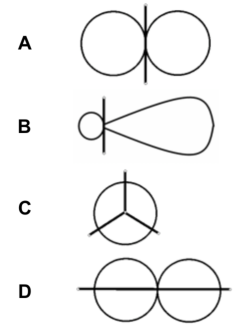
\includegraphics[scale=0.8]{Antennen/Bilder/Strahlungsdiagramm.pdf}
	\caption{Strahlungsdiagramme von Antennen}
	\label{strahlungsdiagramm}
\end{figure}

%------------------------------------------------------

\begin{enumerate} 
\itemsep1pt\parskip0pt\parsep0pt
\item[4] Ordne den Abbildungen \ref{strahlungsdiagramm} folgende Bauformen zu: Groundplane, Yagi-Antenne, Dipol, gibt es nicht.
\loesung{
    Bild A Langdraht
    Bild B Zepelin-Antenne
    Bild C G5RV-Antenne
    Bild D Windom-Antenne
    Bild D Fuchs-Antenne
}
\end{enumerate}
